%*************************************
% ภาคผนวก ก.
%*************************************
\appendixChapterTitle{ก}{การเริ่มต้นใช้งาน MongoDB Atlas}
\vspace*{-0.8in}

% % ใช้ { } ครอบเพื่อบังคับให้การตั้งค่านี้มีผล "แค่หัวข้อนี้หัวข้อเดียว"
% {
%     % ตั้งค่าระยะห่าง: \titlespacing*{คำสั่ง}{ระยะซ้าย}{ระยะบน}{ระยะล่าง}
%     \titlespacing*{\section}{4.8em}{*3}{*2} 
    
%     \section[การสมัครสมาชิกและใช้งาน MongoDB Atlas]{การสมัครสมาชิกและใช้งาน MongoDB Atlas}
% }
% % พอหลุดปีกกา } การตั้งค่าจะกลับเป็นปกติสำหรับหน้าอื่น

\section{การสมัครสมาชิกและใช้งาน MongoDB Atlas}

\hspace*{1.3em}
MongoDB Atlas เป็นบริการ Database-as-a-Service (DBaaS) ของ MongoDB ที่ให้บริการ cloud database แบบ fully managed รองรับการใช้งานบน AWS, Google Cloud และ Azure โดยมีจุดเด่นคือช่วยลดภาระของผู้พัฒนาในการติดตั้งและดูแลรักษาเซิร์ฟเวอร์ฐานข้อมูล (Server Maintenance) อีกทั้งยังมีระบบรักษาความปลอดภัยที่ได้มาตรฐาน มีระบบสำรองข้อมูลอัตโนมัติ และรองรับการขยายขนาด (Scalability) ได้ง่ายเมื่อข้อมูลมีปริมาณมากขึ้น

\begin{figure}[H]
\centering
\adjustbox{frame, width=1\textwidth}{
    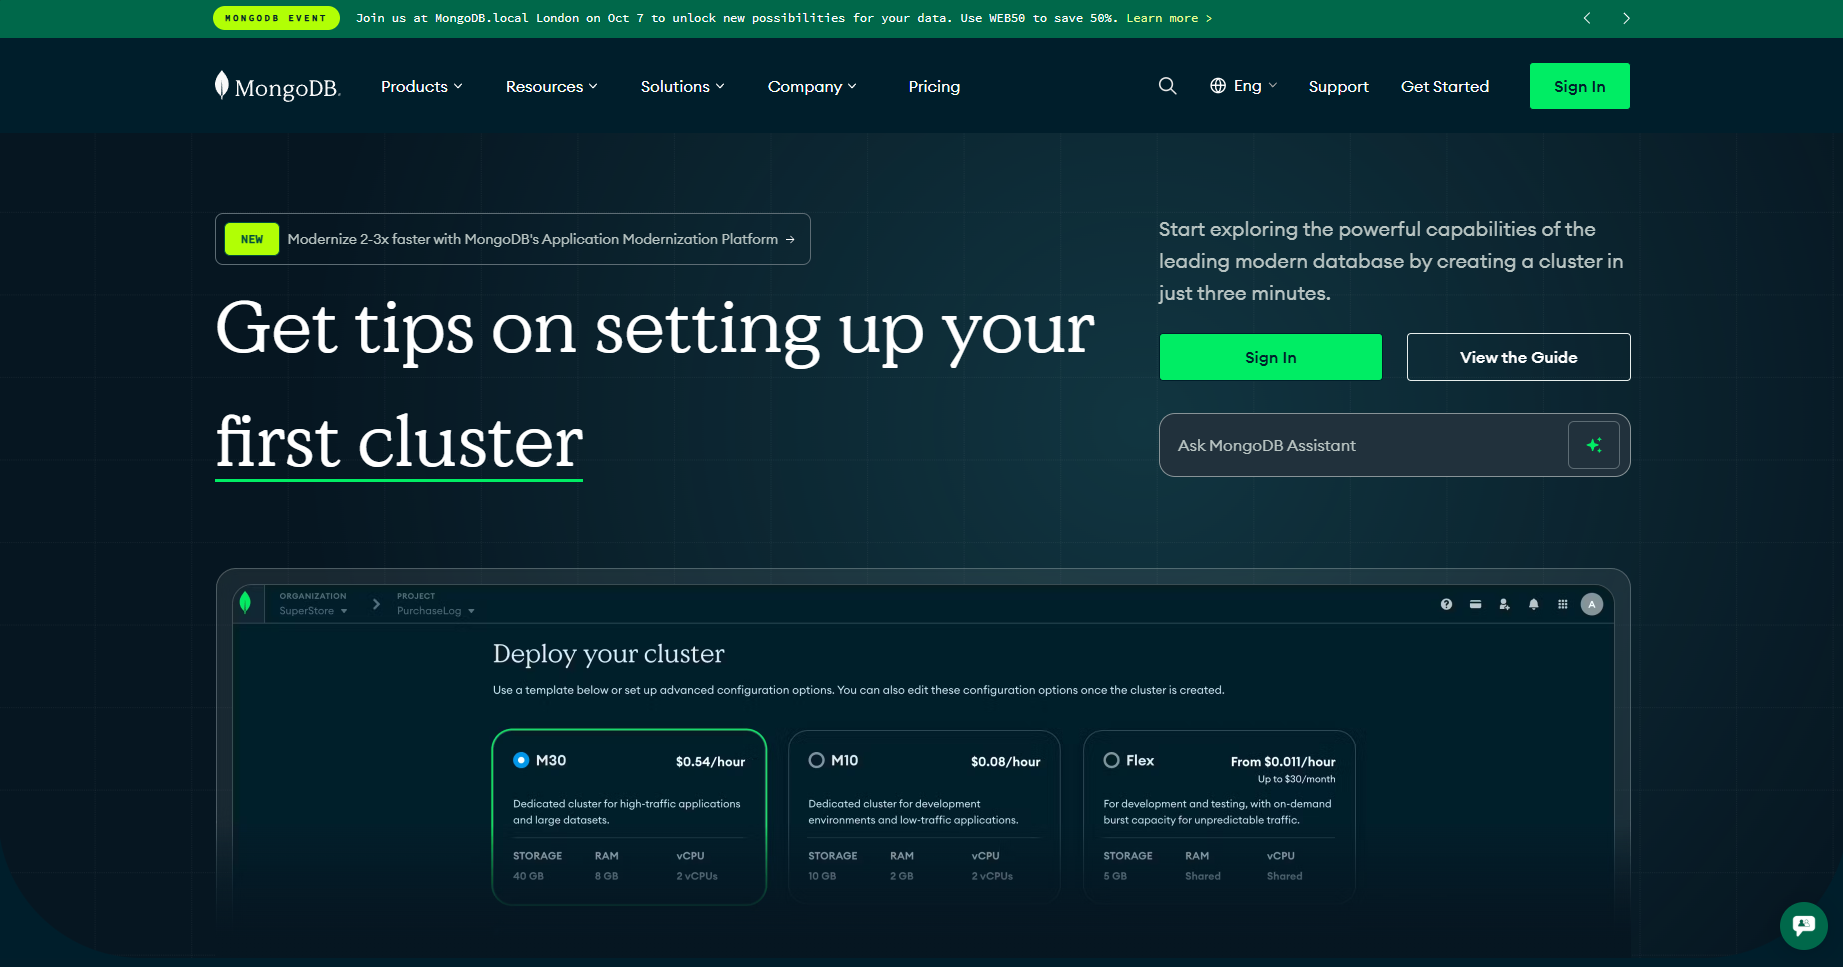
\includegraphics[width=1\textwidth]{Image/mongodb-page.png}
}
\caption{\fontSixTeen{หน้าแรกของเว็บไซต์ MongoDB}}
\label{figA:WebSiteMongoDB1}
\end{figure}
\begin{mycustomenum2}
    \item ไปที่เว็บไซต์ MongoDB (\href{https://www.mongodb.com/}{www.mongodb.com}) ตัวอย่างหน้าเว็บไซต์ MongoDB แสดงได้ดังภาพที่ \ref{figA:WebSiteMongoDB1}
    \item ที่หน้าแรกดังภาพที่ \ref{figA:WebSiteMongoDB1} ในกรณีที่ยังไม่ได้เป็นสมาชิกให้คลิกที่ \enquote{Get Started} ก็จะพบกับหน้าจอดังภาพที่ \ref{figA:WebSiteMongoDB2}

\hspace*{1.3em}

\hspace*{1.3em}

\vspace*{-0.6in}
\begin{figure}[H]
\centering
\adjustbox{frame, width=1.0\textwidth}{
    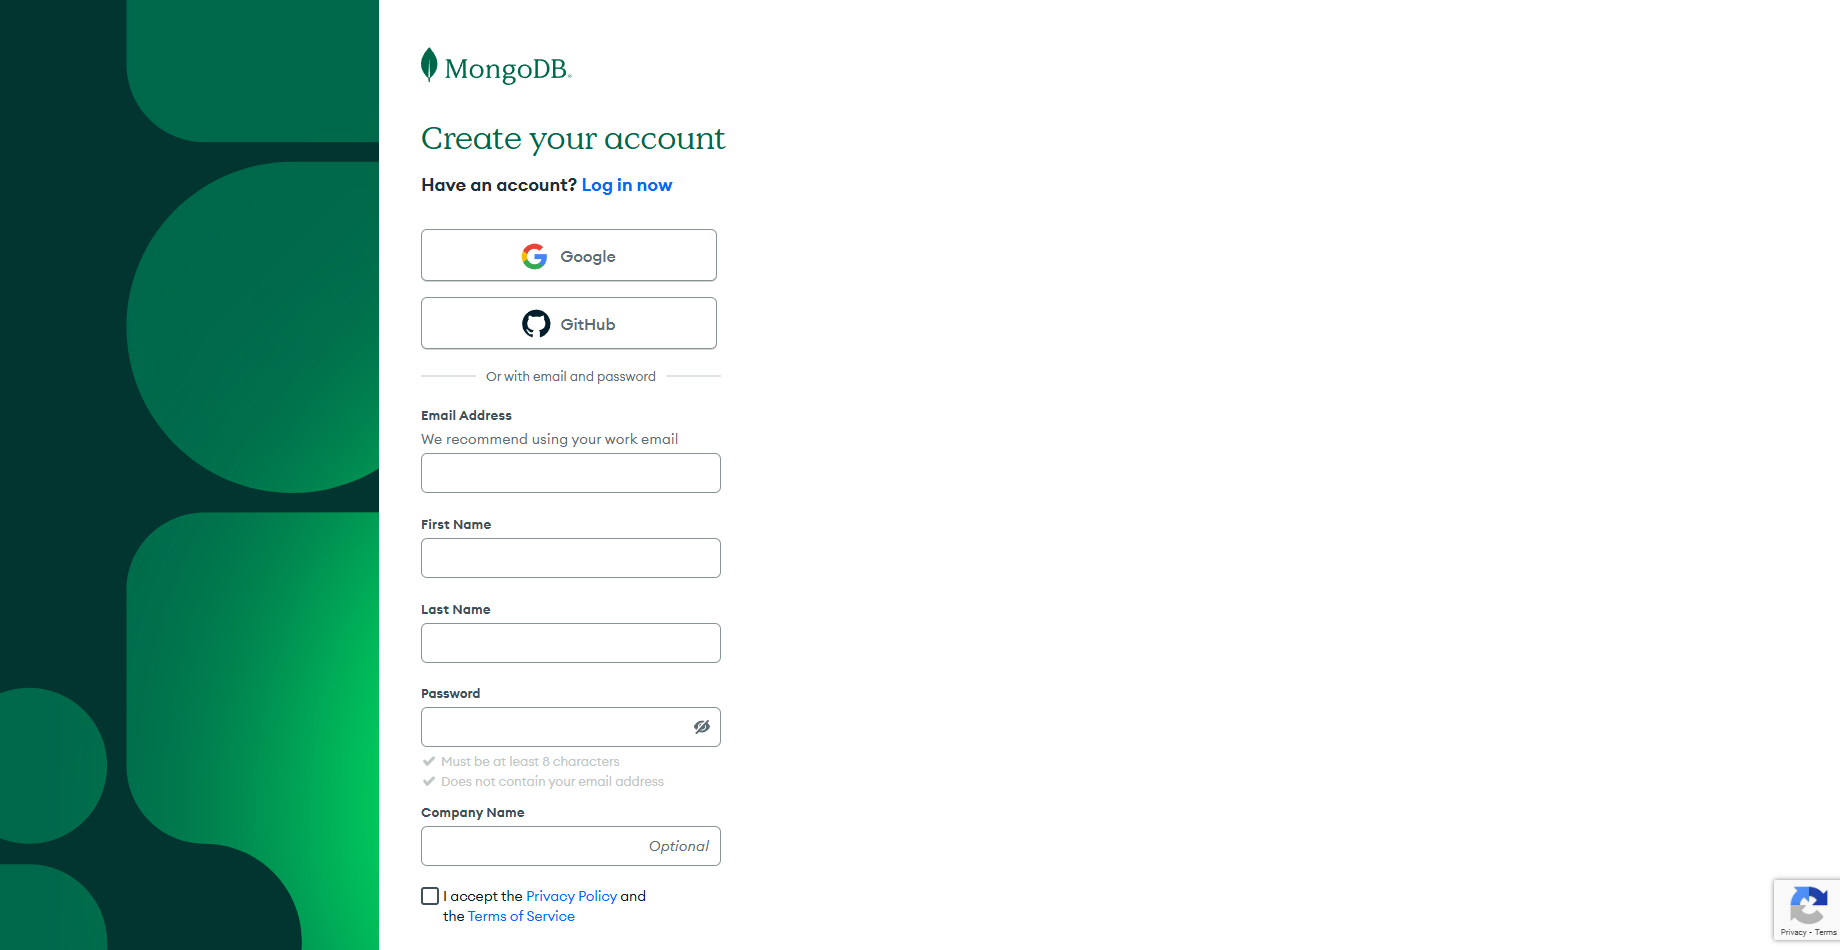
\includegraphics[width=1.0\textwidth]{Image/mongodb-regis.png}
}
\caption{\fontSixTeen{หน้า Sign up ของเว็บไซต์ MongoDB}}
\label{figA:WebSiteMongoDB2}
\end{figure}
  \item ผู้ใช้งานสามารถเลือกสมัครสมาชิกได้หลายวิธี เช่น
    \begin{mycustomenum2}
        \item สมัครด้วยอีเมล โดยกรอกชื่อ อีเมล และรหัสผ่านที่ต้องการ
        \item สมัครด้วย Google mail ซึ่งเป็นวิธีที่ง่ายและรวดเร็ว
        \item สมัครด้วย GitHub
    \end{mycustomenum2}     


\begin{figure}[H]
\centering
\adjustbox{frame, width=1.0\textwidth}{
    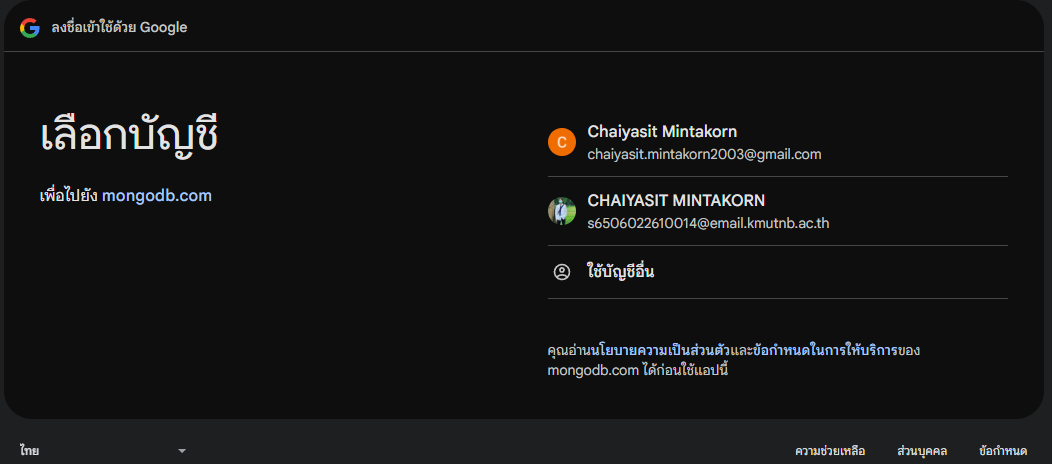
\includegraphics[width=1.0\textwidth]{Image/mongodb-select.png}
}
\caption{\fontSixTeen{หน้าเลือกบัญชี Google สำหรับสมัครสมาชิกด้วย Google mail}}
\label{figA:WebSiteMongoDB3}
\end{figure}
    \item เลือก Gmail ที่ต้องการใช้สมัครสมาชิก

\vspace*{-0.7in}
\begin{figure}[H]
\centering
\adjustbox{frame, width=1.0\textwidth}{
    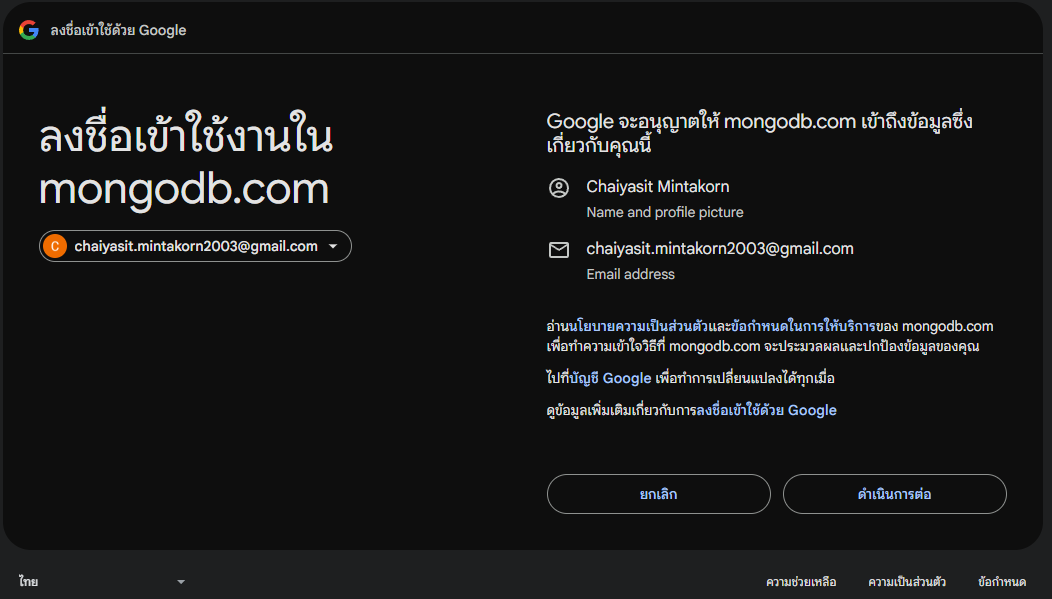
\includegraphics[width=1.0\textwidth]{Image/mongodb-google.png}
}
\caption{\fontSixTeen{หน้ายืนยันให้ MongoDB เข้าถึงข้อมูล}}
\label{figA:WebSiteMongoDB4}
\end{figure}

\begin{figure}[H]
\centering
\adjustbox{frame, width=1.0\textwidth}{
    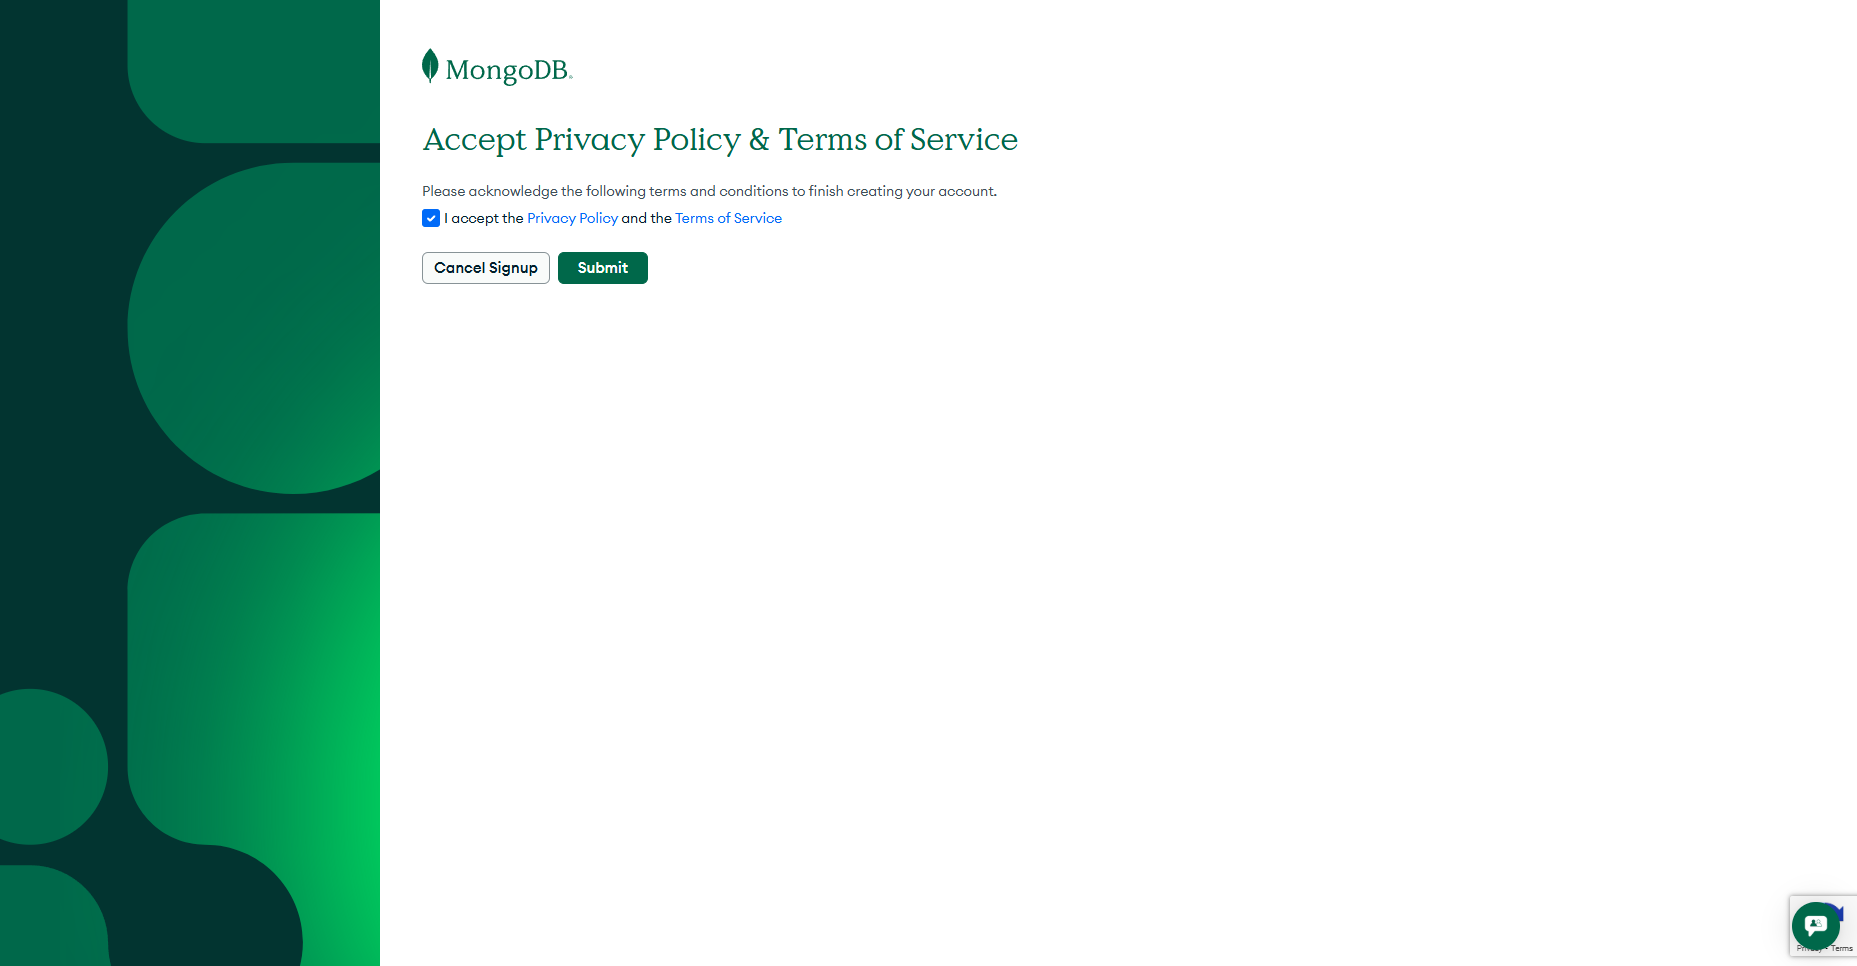
\includegraphics[width=1.0\textwidth]{Image/mongodb-policy.png}
}
\caption{\fontSixTeen{หน้าเว็บไซต์ MongoDB อนุญาตให้เข้าถึงข้อมูลส่วนตัว}}
\label{figA:WebSiteMongoDB5}
\end{figure}

\vspace*{-0.6in}
\begin{figure}[H]
\centering
\adjustbox{frame, width=1.0\textwidth}{
    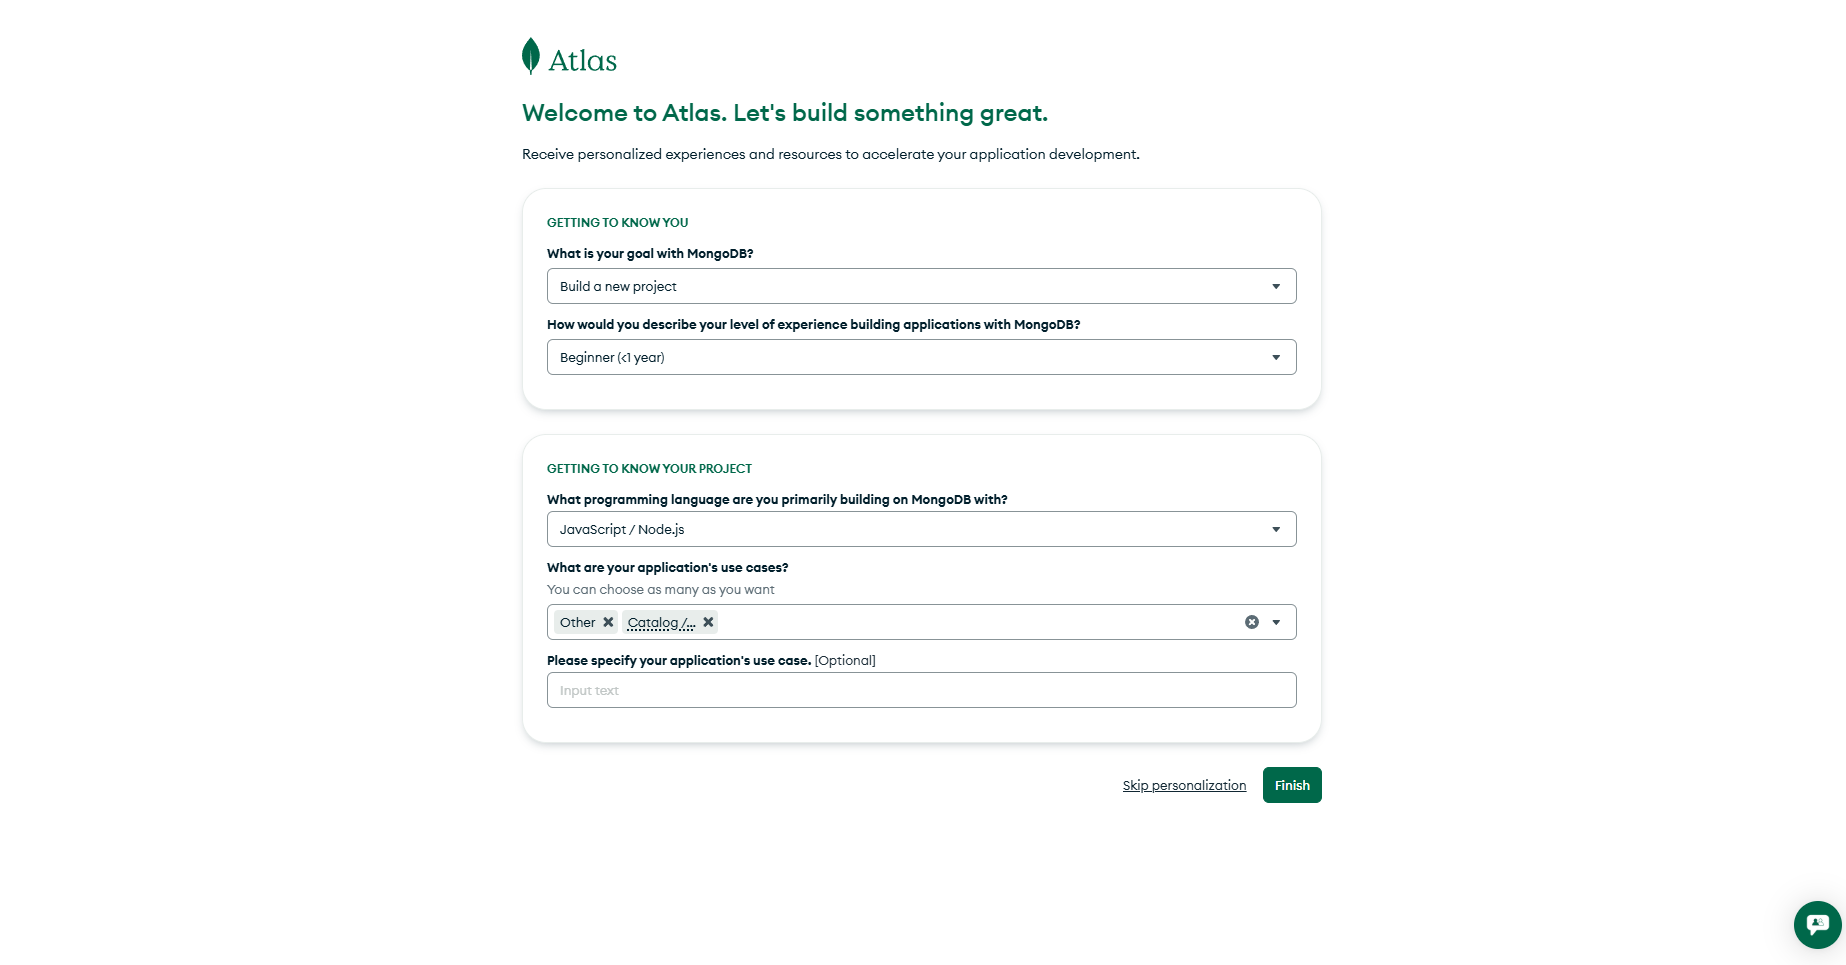
\includegraphics[width=1.0\textwidth]{Image/mongodb-personal.png}
}
\caption{\fontSixTeen{หน้าเพิ่มข้อมูลส่วนตัว}}
\label{figA:WebSiteMongoDB6}
\end{figure}
    \item หลังจากเพิ่มข้อมูลส่วนตัวแล้วคลิกที่ \enquote{Finish} หรือคลิกที่ \enquote{Skip personalization} เพื่อข้ามไปหน้าถัดไป

\begin{figure}[H]
\centering
\adjustbox{frame, width=1.0\textwidth}{
    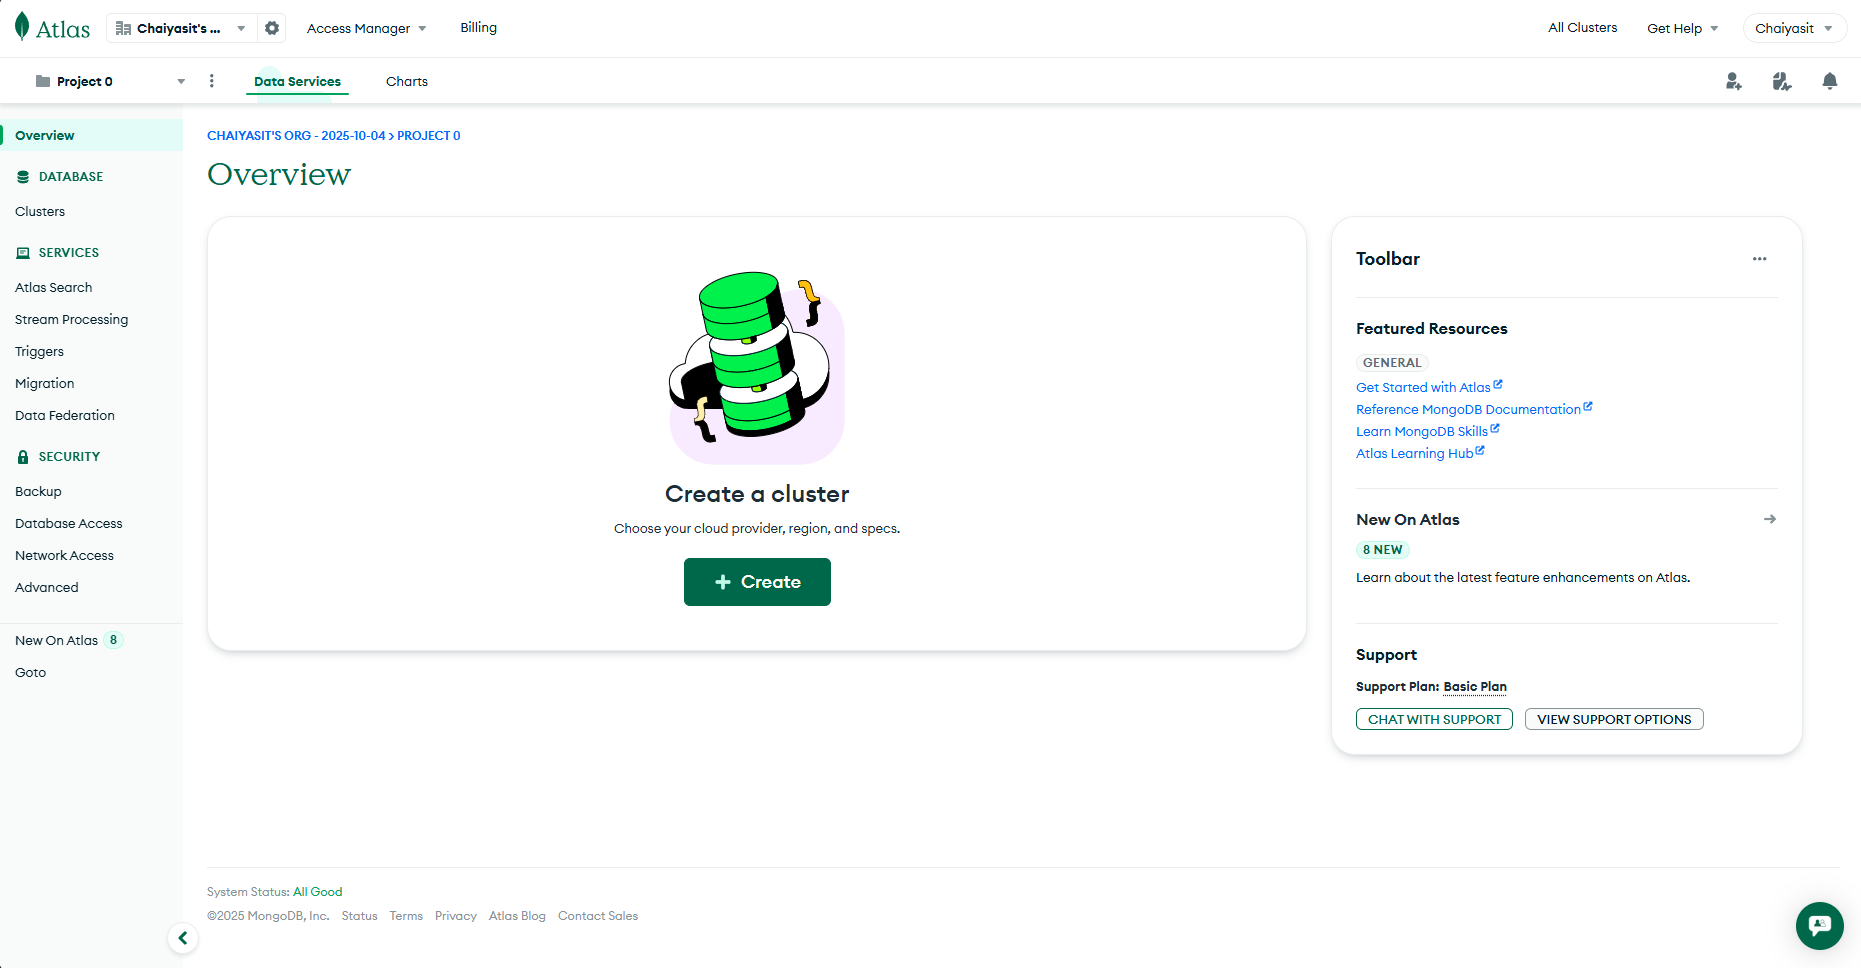
\includegraphics[width=1.0\textwidth]{Image/mongodb-overview.png}
}
\caption{\fontSixTeen{หน้าแรกหลังจากลงทะเบียนเว็บไซต์ MongoDB สำเร็จแล้ว}}
\label{figA:WebSiteMongoDB7}
\end{figure}       

\vspace*{-0.6in}
\begin{figure}[H]
\centering
\adjustbox{frame, width=1.0\textwidth}{
    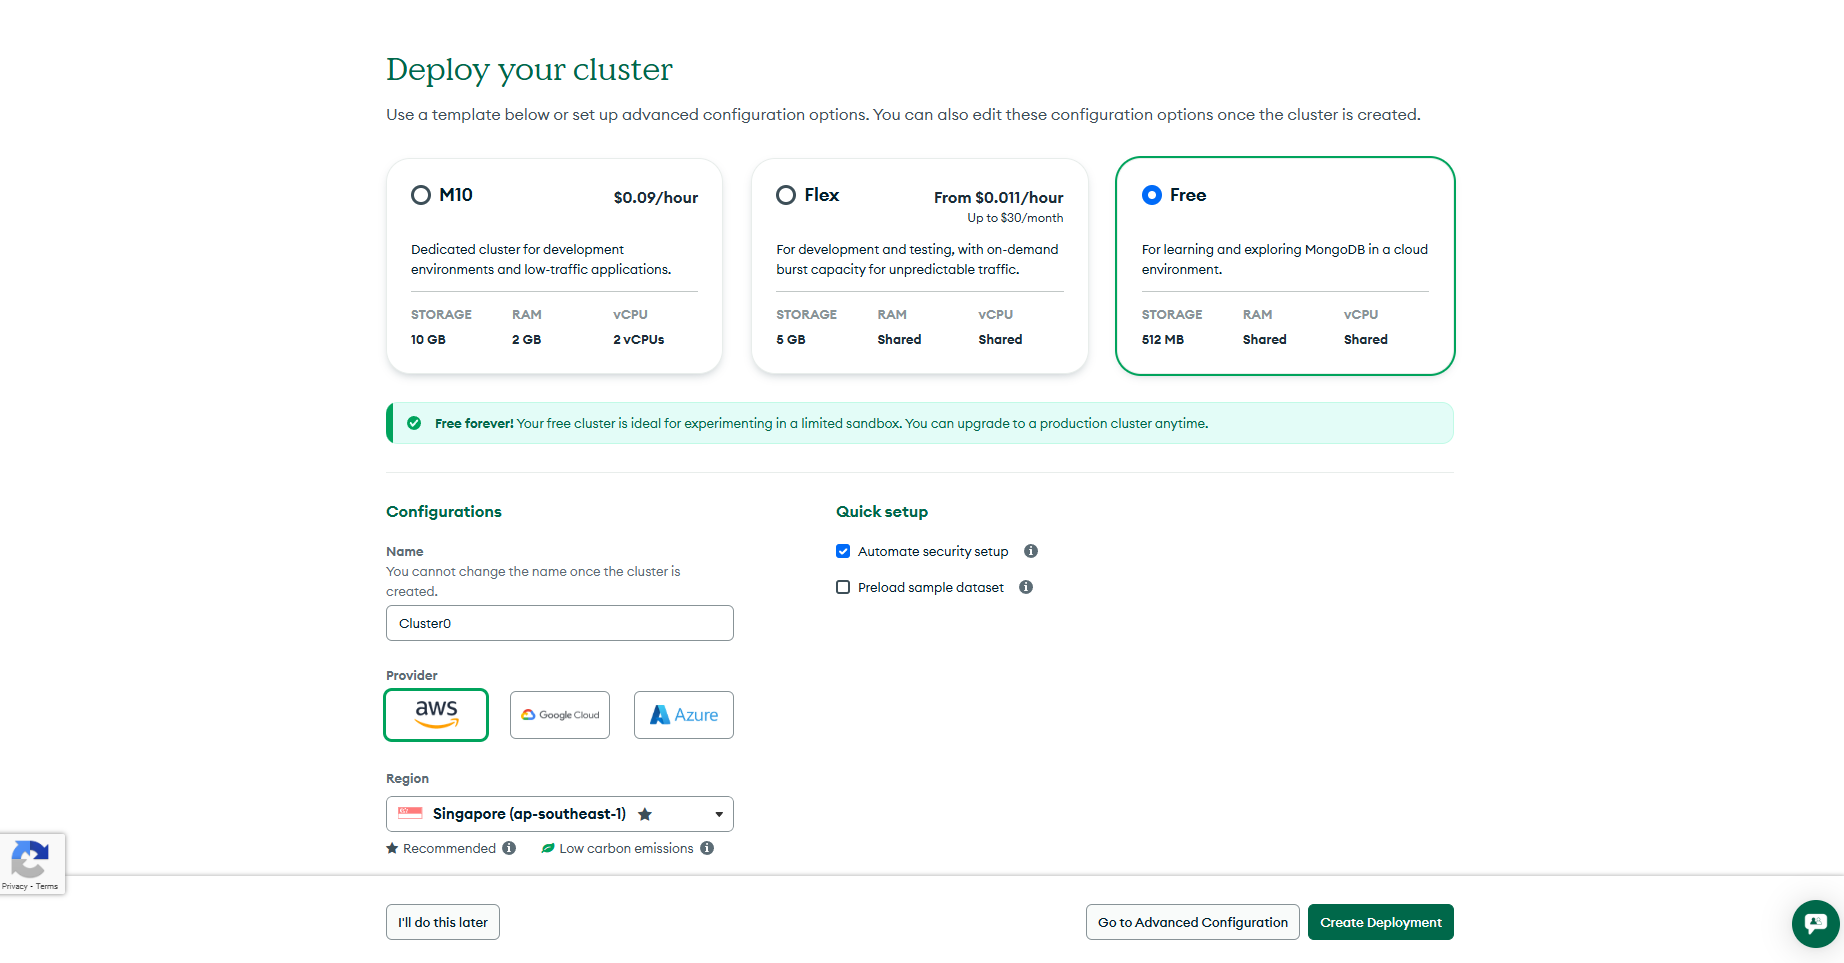
\includegraphics[width=1.0\textwidth]{Image/mongodb-cluster.png}
}
\caption{\fontSixTeen{หน้าสำหรับสร้าง Cluster ใน MongoDB}}
\label{figA:WebSiteMongoDB8}
\end{figure}
    \item จากภาพที่ \ref{figA:WebSiteMongoDB7} คลิกที่ \enquote{Create} ก็จะพบกับหน้าจอดังภาพที่ \ref{figA:WebSiteMongoDB8} สามารถเลือกรูปแบบการ Deploy ได้ ในที่นี้เลือก Free จากนั้นให้ตั้งชื่อ Cluster และกดคลิกที่ \enquote{Create Deployment}  

\begin{figure}[H]
\centering
\adjustbox{frame, width=1.0\textwidth}{
    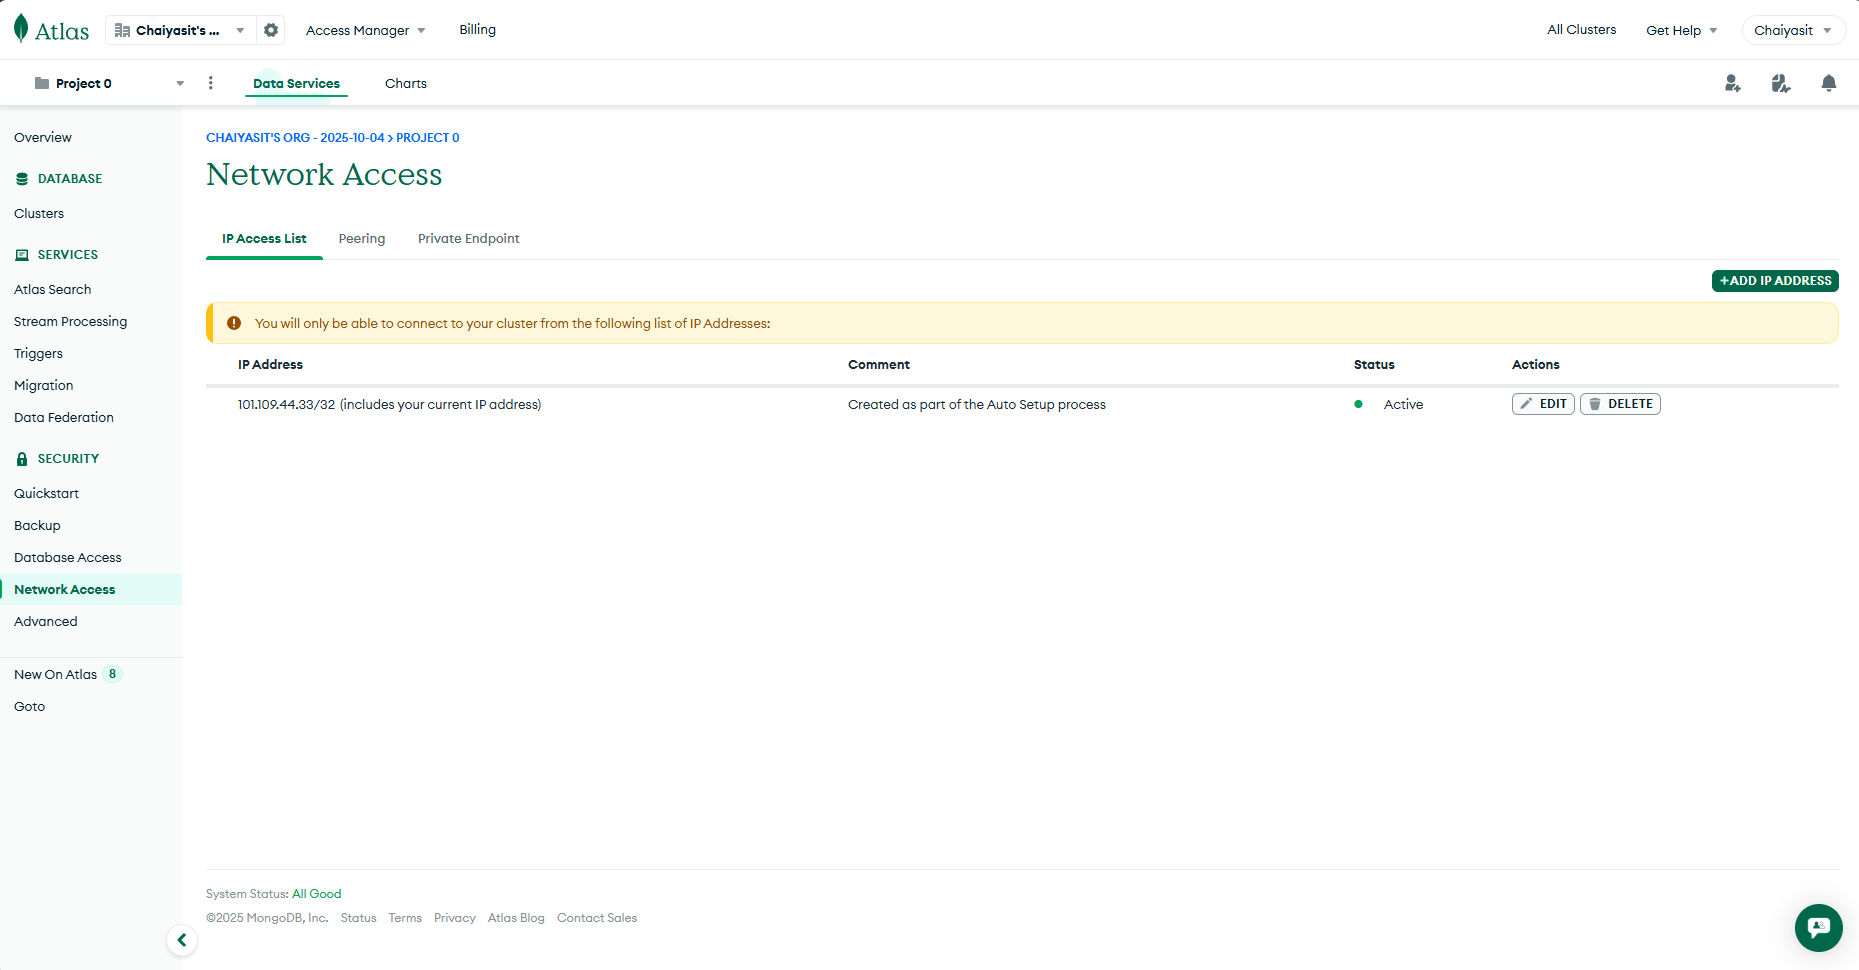
\includegraphics[width=1.0\textwidth]{Image/mongodb-ip.png}
}
\caption{\fontSixTeen{หน้าสำหรับการแก้ไข IP Address ที่อนุญาตให้เข้าถึง Cluster}}
\label{figA:WebSiteMongoDB9}
\end{figure}

    \item จากภาพที่ \ref{figA:WebSiteMongoDB7} ให้คลิกที่ \enquote{Network Access} ที่เมนูด้านซ้าย และคลิกที่ \enquote{Add IP Address} ก็จะพบกับหน้าจอดังภาพที่ \ref{figA:WebSiteMongoDB10} 

\vspace*{-0.6in}
\begin{figure}[H]
\centering
\adjustbox{frame, width=1.0\textwidth}{
    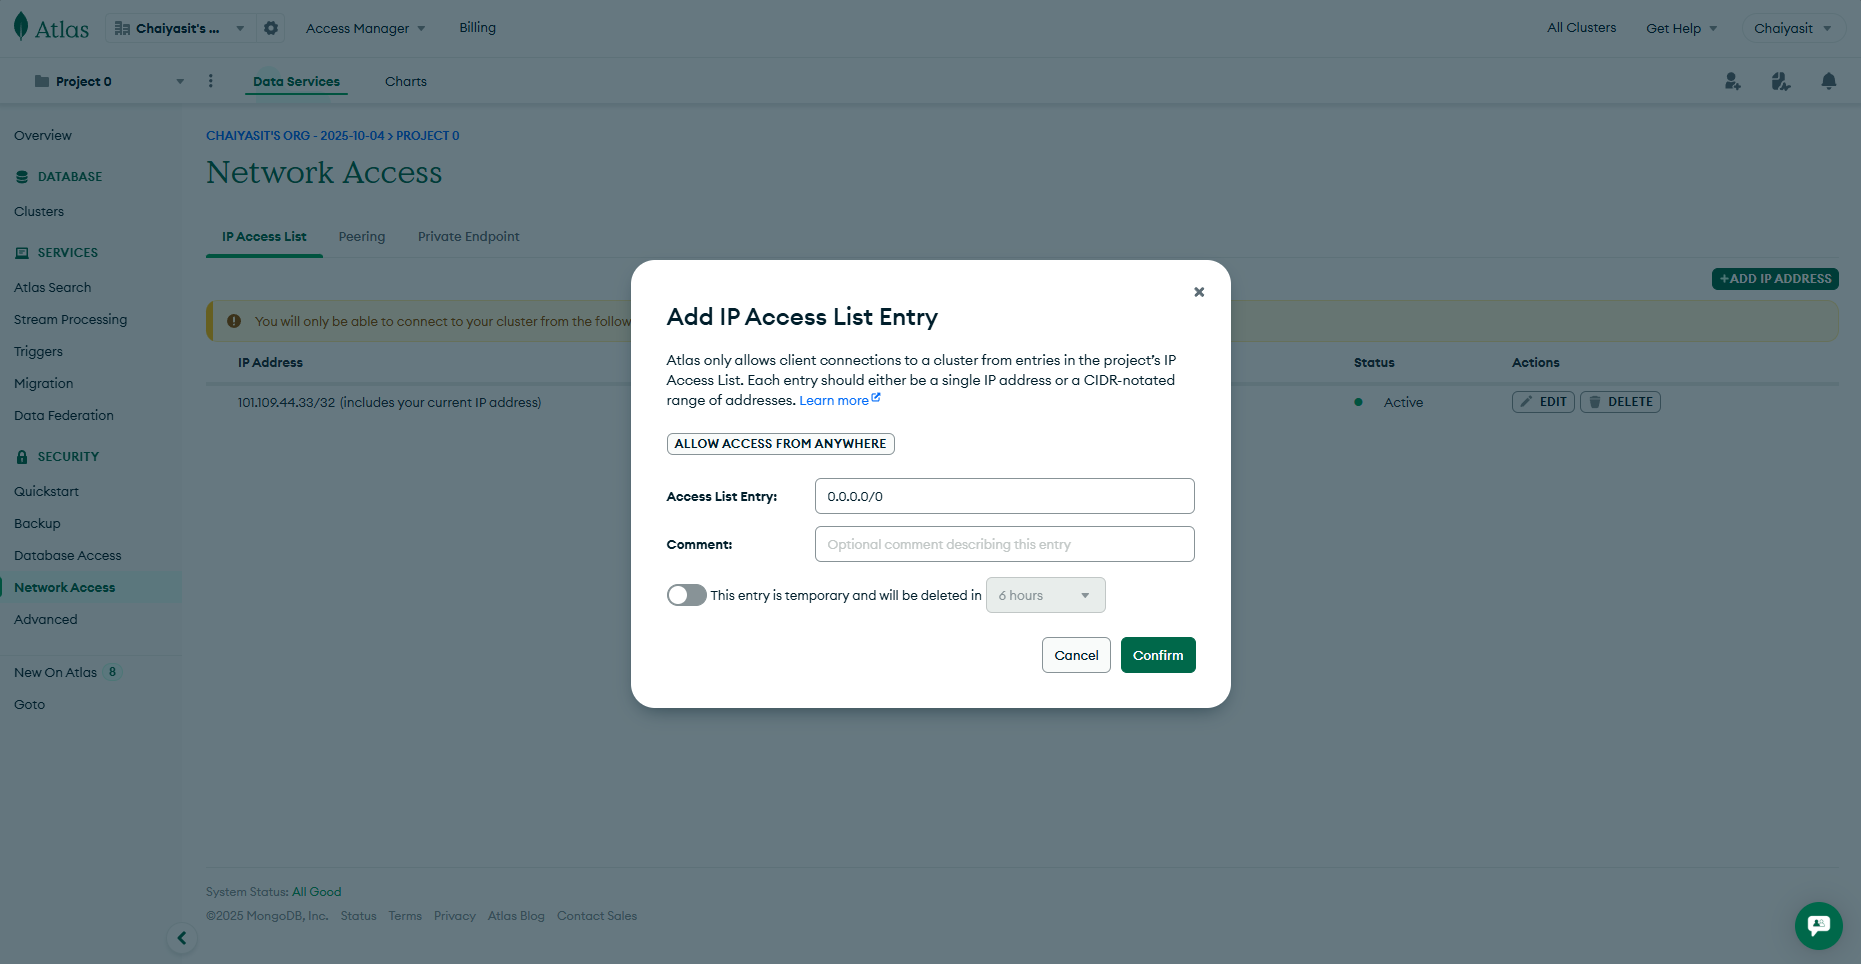
\includegraphics[width=1.0\textwidth]{Image/mongodb-add-ip.png}
}
\caption{\fontSixTeen{หน้าสำหรับเพิ่ม IP Address ที่อนุญาตให้เข้าถึง Cluster}}
\label{figA:WebSiteMongoDB10}
\end{figure}

    \item จากภาพที่ \ref{figA:WebSiteMongoDB10} ให้คลิกที่ \enquote{Allow Access from Anywhere} เพื่ออนุญาตให้ทุก IP Address สามารถเข้าถึง Cluster ได้ จากนั้นคลิกที่ \enquote{Confirm} ก็จะพบกับหน้าจอดังภาพที่ \ref{figA:WebSiteMongoDB11}

\begin{figure}[H]
\centering
\adjustbox{frame, width=1.0\textwidth}{
    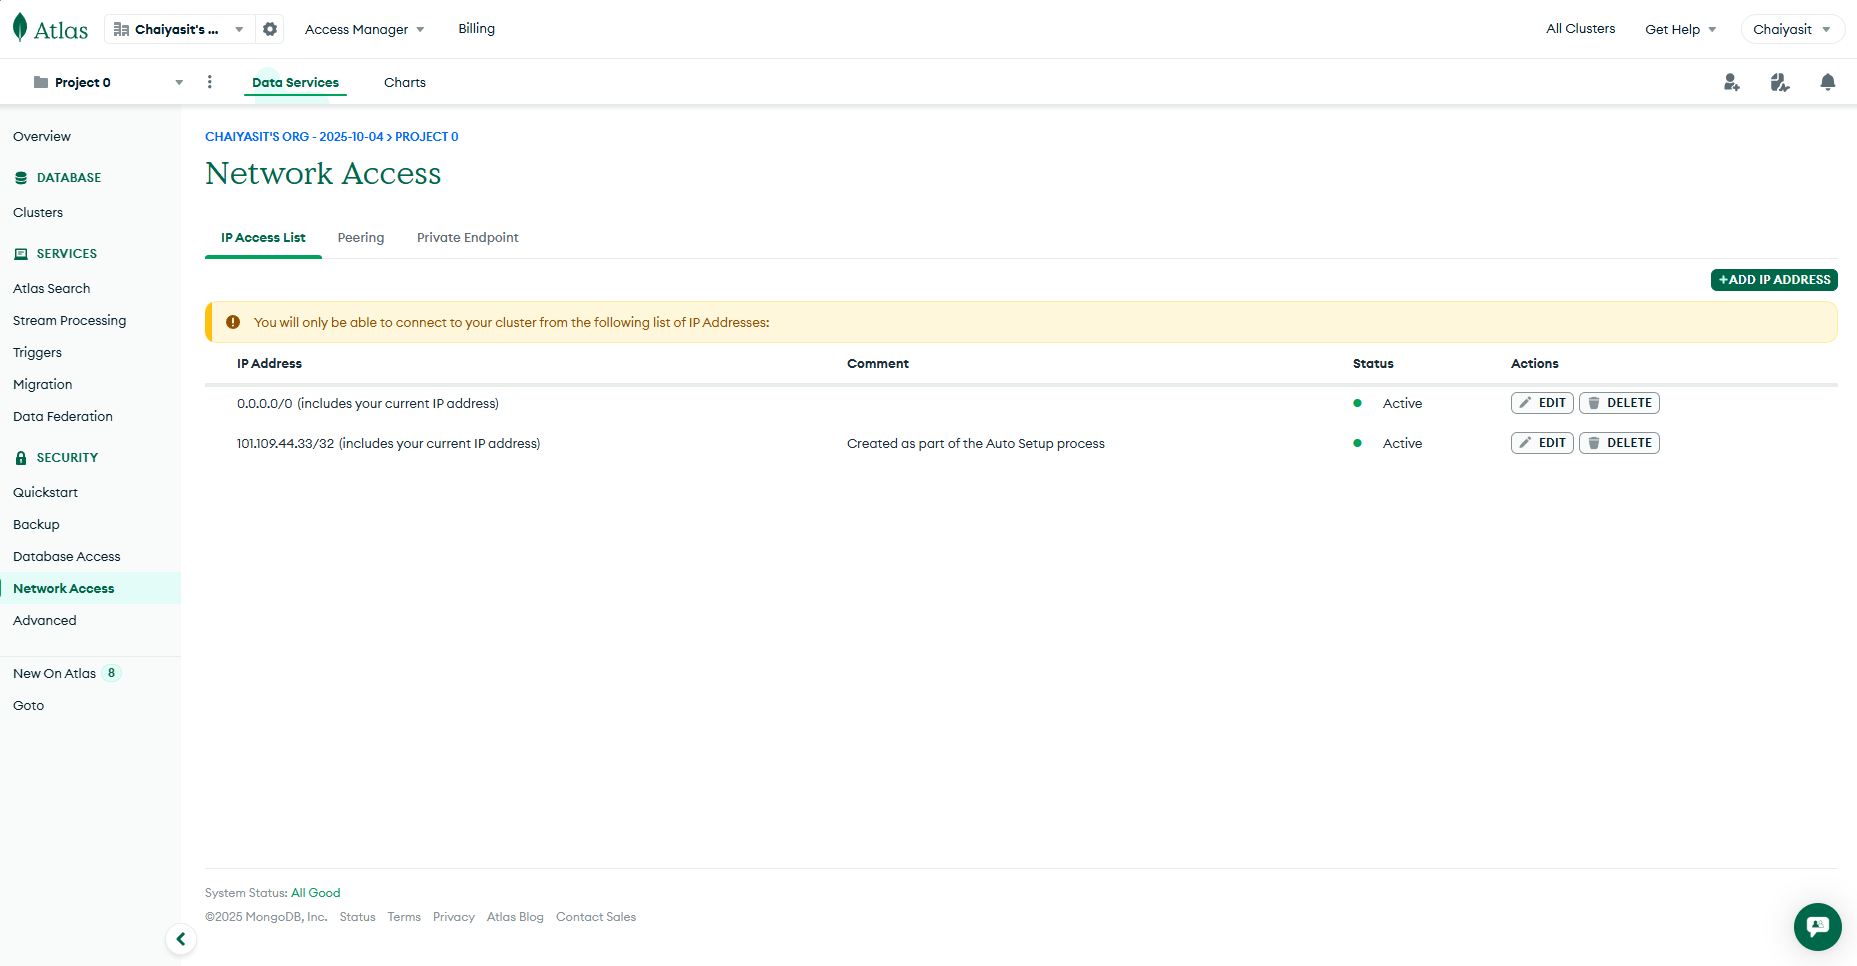
\includegraphics[width=1.0\textwidth]{Image/mongodb-ip-list.png}
}
\caption{\fontSixTeen{หน้าแสดงรายการ IP Address ที่อนุญาตให้เข้าถึง Cluster}}
\label{figA:WebSiteMongoDB11}
\end{figure}

\vspace*{-0.6in}
\begin{figure}[H]
\centering
\adjustbox{frame, width=1.0\textwidth}{
    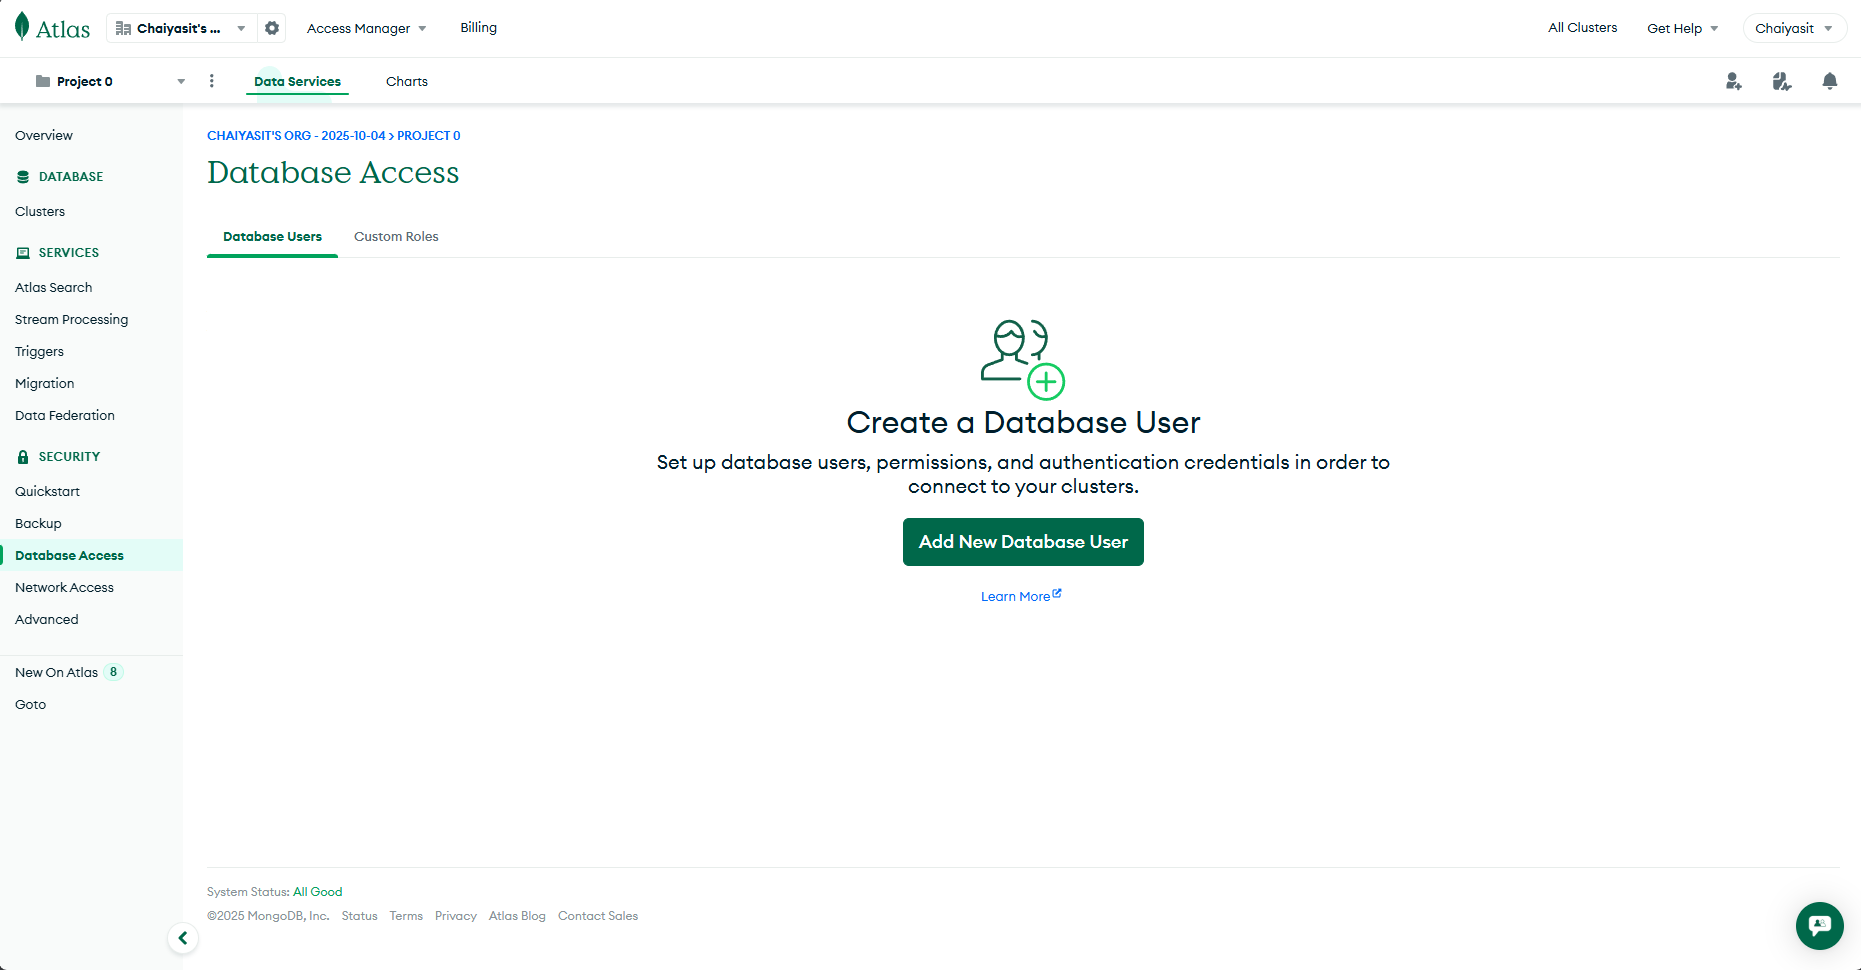
\includegraphics[width=1.0\textwidth]{Image/mongodb-add-user.png}
}
\caption{\fontSixTeen{หน้าสำหรับเพิ่มผู้ใช้งานที่สามารถเข้าถึง Cluster}}
\label{figA:WebSiteMongoDB12}
\end{figure}
    \item จากภาพที่ \ref{figA:WebSiteMongoDB7} ที่เมนูด้านซ้ายให้คลิกที่ \enquote{Database Access} และคลิกที่ \enquote{Add New Database User} ก็จะพบกับหน้าจอดังภาพที่ \ref{figA:WebSiteMongoDB12}

\begin{figure}[H]
\centering
\adjustbox{frame, width=1.0\textwidth}{
    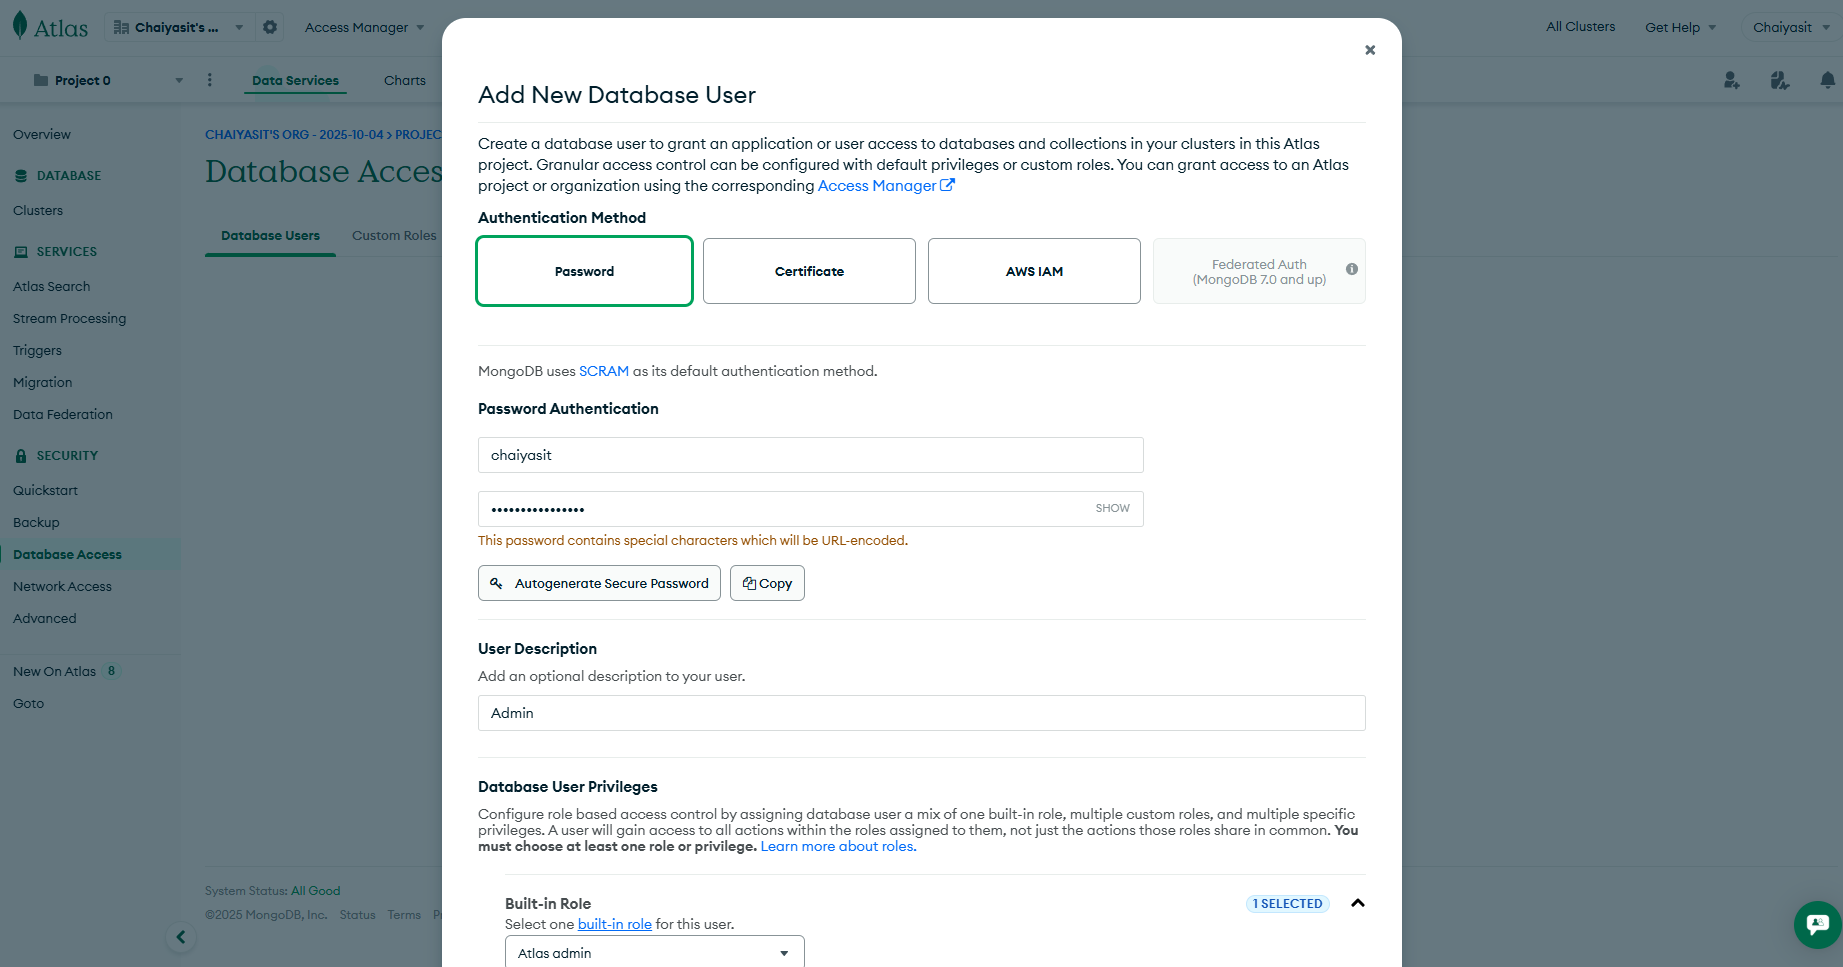
\includegraphics[width=1.0\textwidth]{Image/mongodb-add-user2.png}
}
\caption{\fontSixTeen{หน้าเพิ่มผู้ใช้งานที่สามารถเข้าถึง Cluster}}
\label{figA:WebSiteMongoDB13}
\end{figure}
    \item จากภาพที่ \ref{figA:WebSiteMongoDB13} ใส่ Username และ Password ที่ต้องการ จากนั้นคลิกที่ \enquote{Add User} ก็จะพบกับหน้าจอดังภาพที่ \ref{figA:WebSiteMongoDB14}

\vspace*{-0.6in}
\begin{figure}[H]
\centering
\adjustbox{frame, width=1.0\textwidth}{
    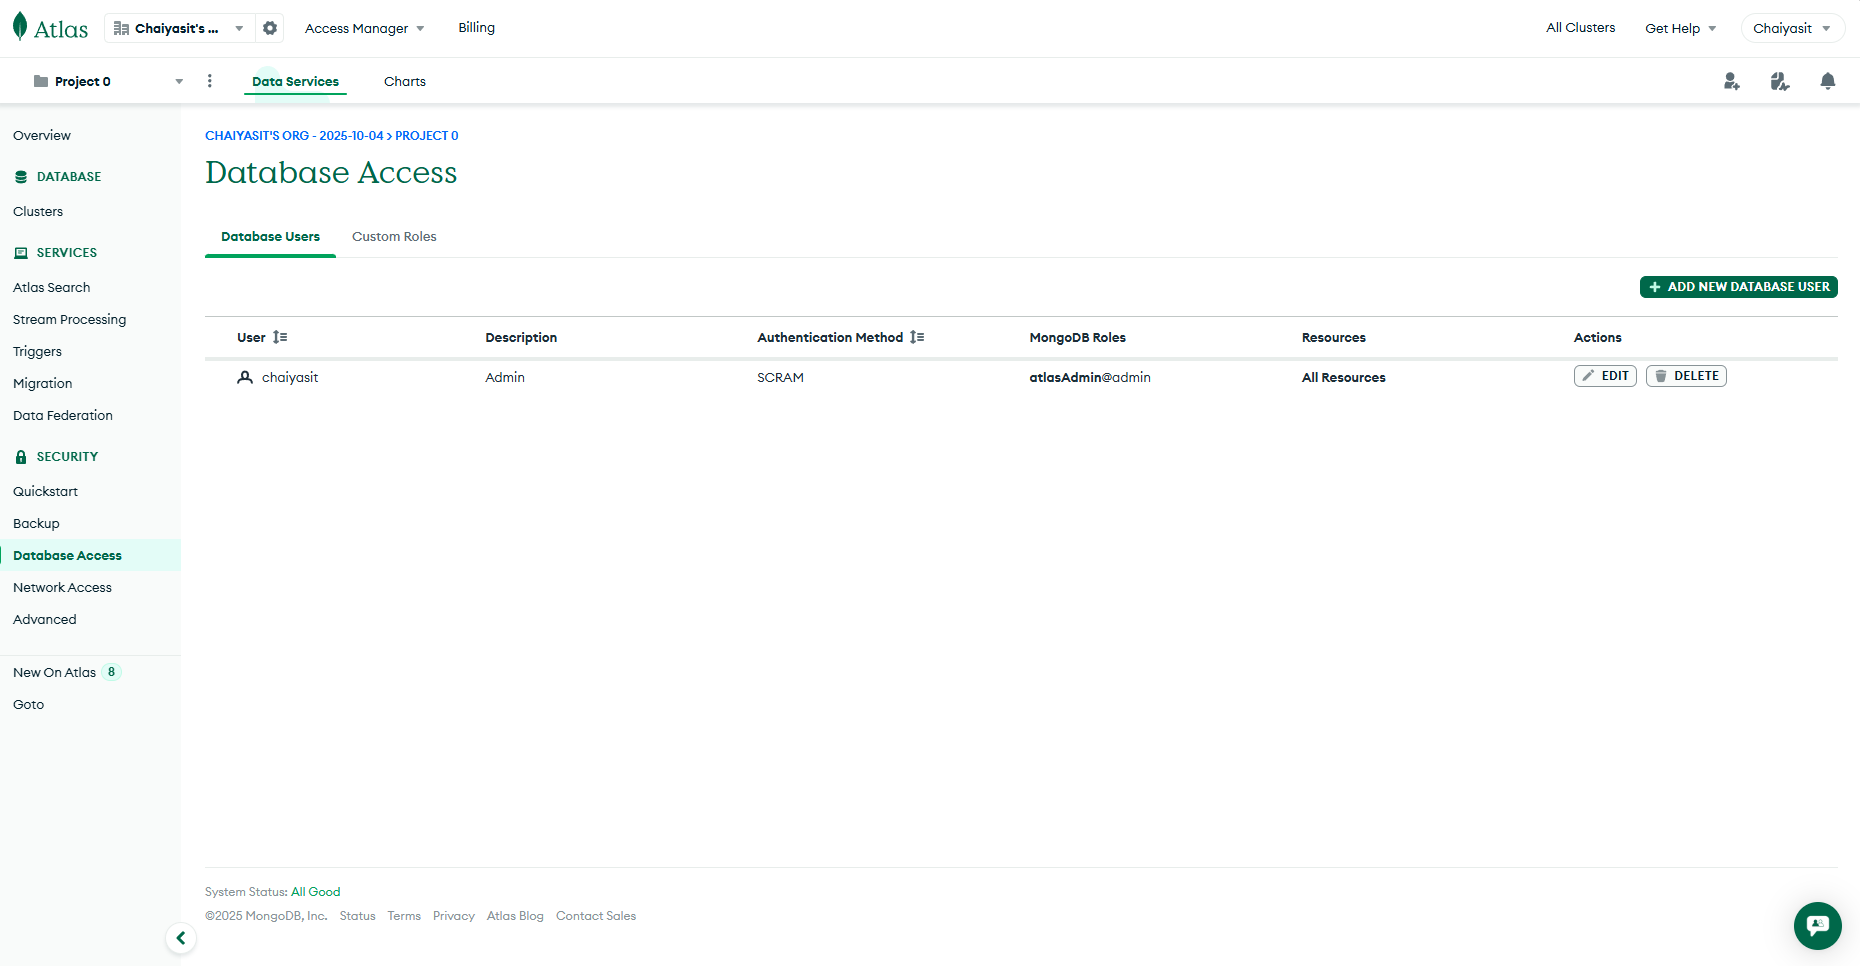
\includegraphics[width=1.0\textwidth]{Image/mongodb-add-user3.png}
}
\caption{\fontSixTeen{หน้าแสดงรายชื่อผู้ใช้งานที่สามารถเข้าถึง Cluster}}
\label{figA:WebSiteMongoDB14}
\end{figure}

\begin{figure}[H]
\centering
\adjustbox{frame, width=1.0\textwidth}{
    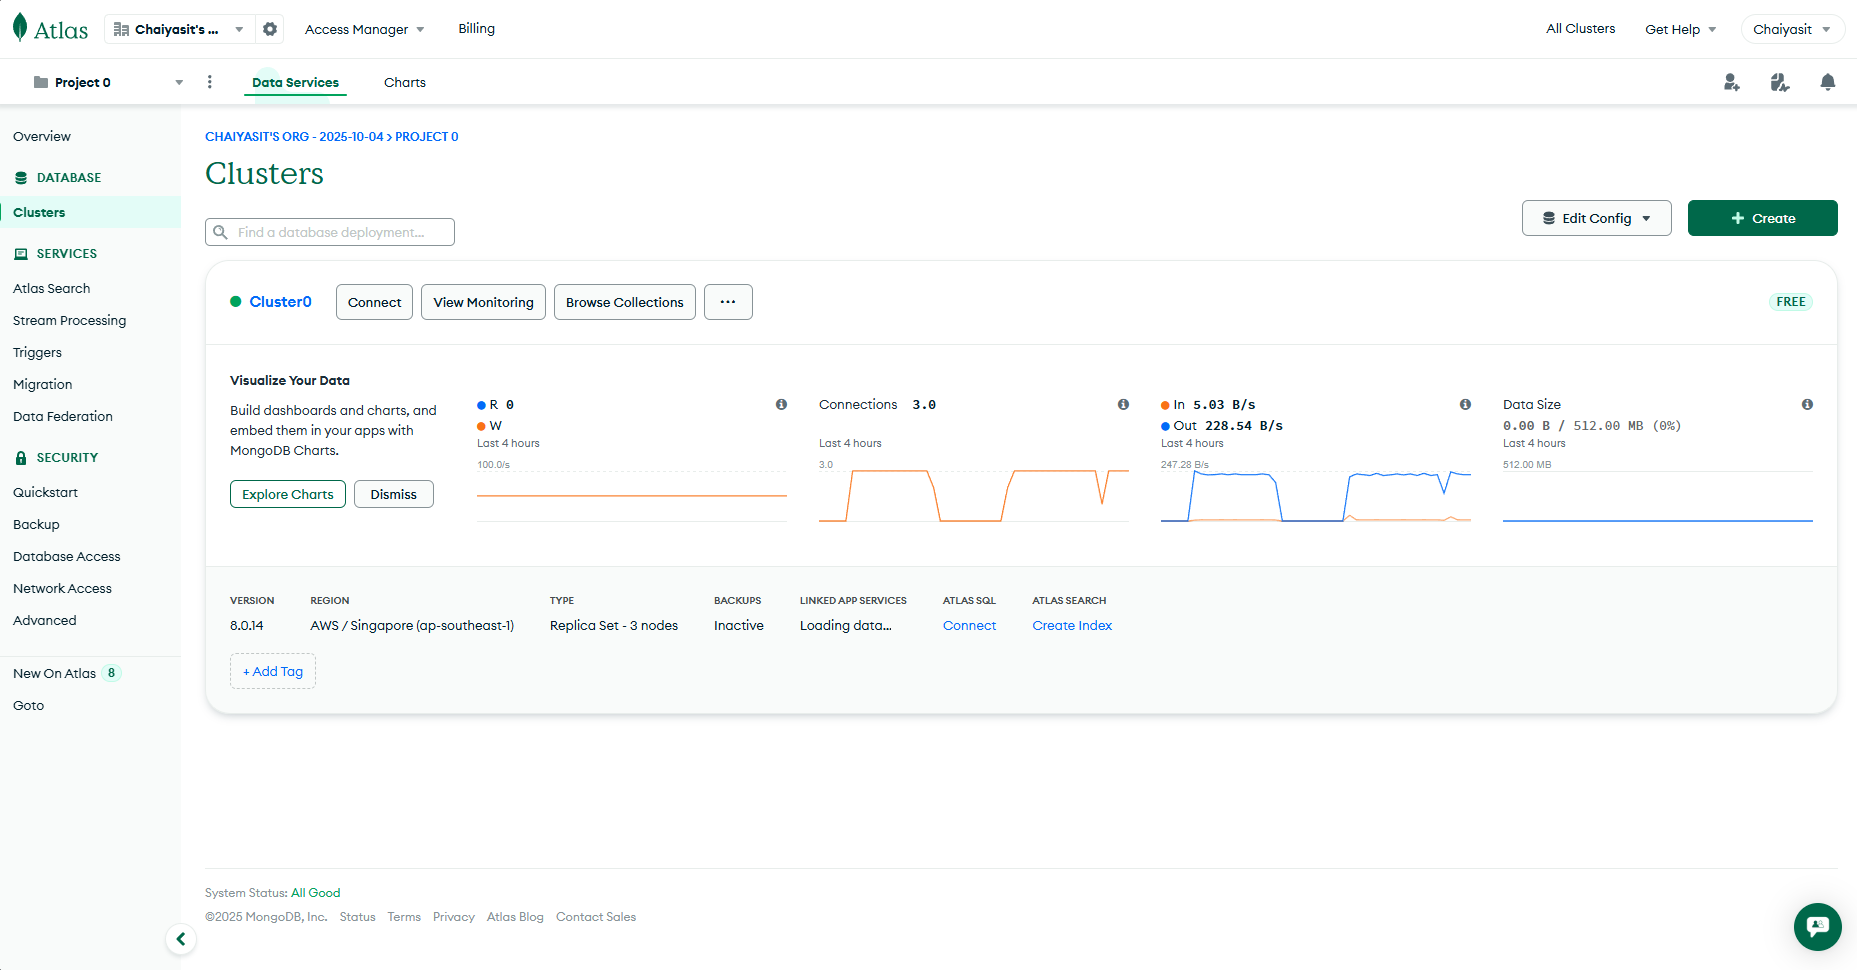
\includegraphics[width=1.0\textwidth]{Image/mongodb-use.png}
}
\caption{\fontSixTeen{หน้าแสดงรายละเอียด Cluster}}
\label{figA:WebSiteMongoDB15}
\end{figure}
    \item จากภาพที่ \ref{figA:WebSiteMongoDB7} ที่เมนูด้านซ้ายให้คลิกที่ \enquote{Cluster} และคลิกที่ \enquote{Connect} ก็จะพบกับหน้าจอดังภาพที่ \ref{figA:WebSiteMongoDB16}

\vspace*{-0.6in}
\begin{figure}[H]
\centering
\adjustbox{frame, width=1.0\textwidth}{
    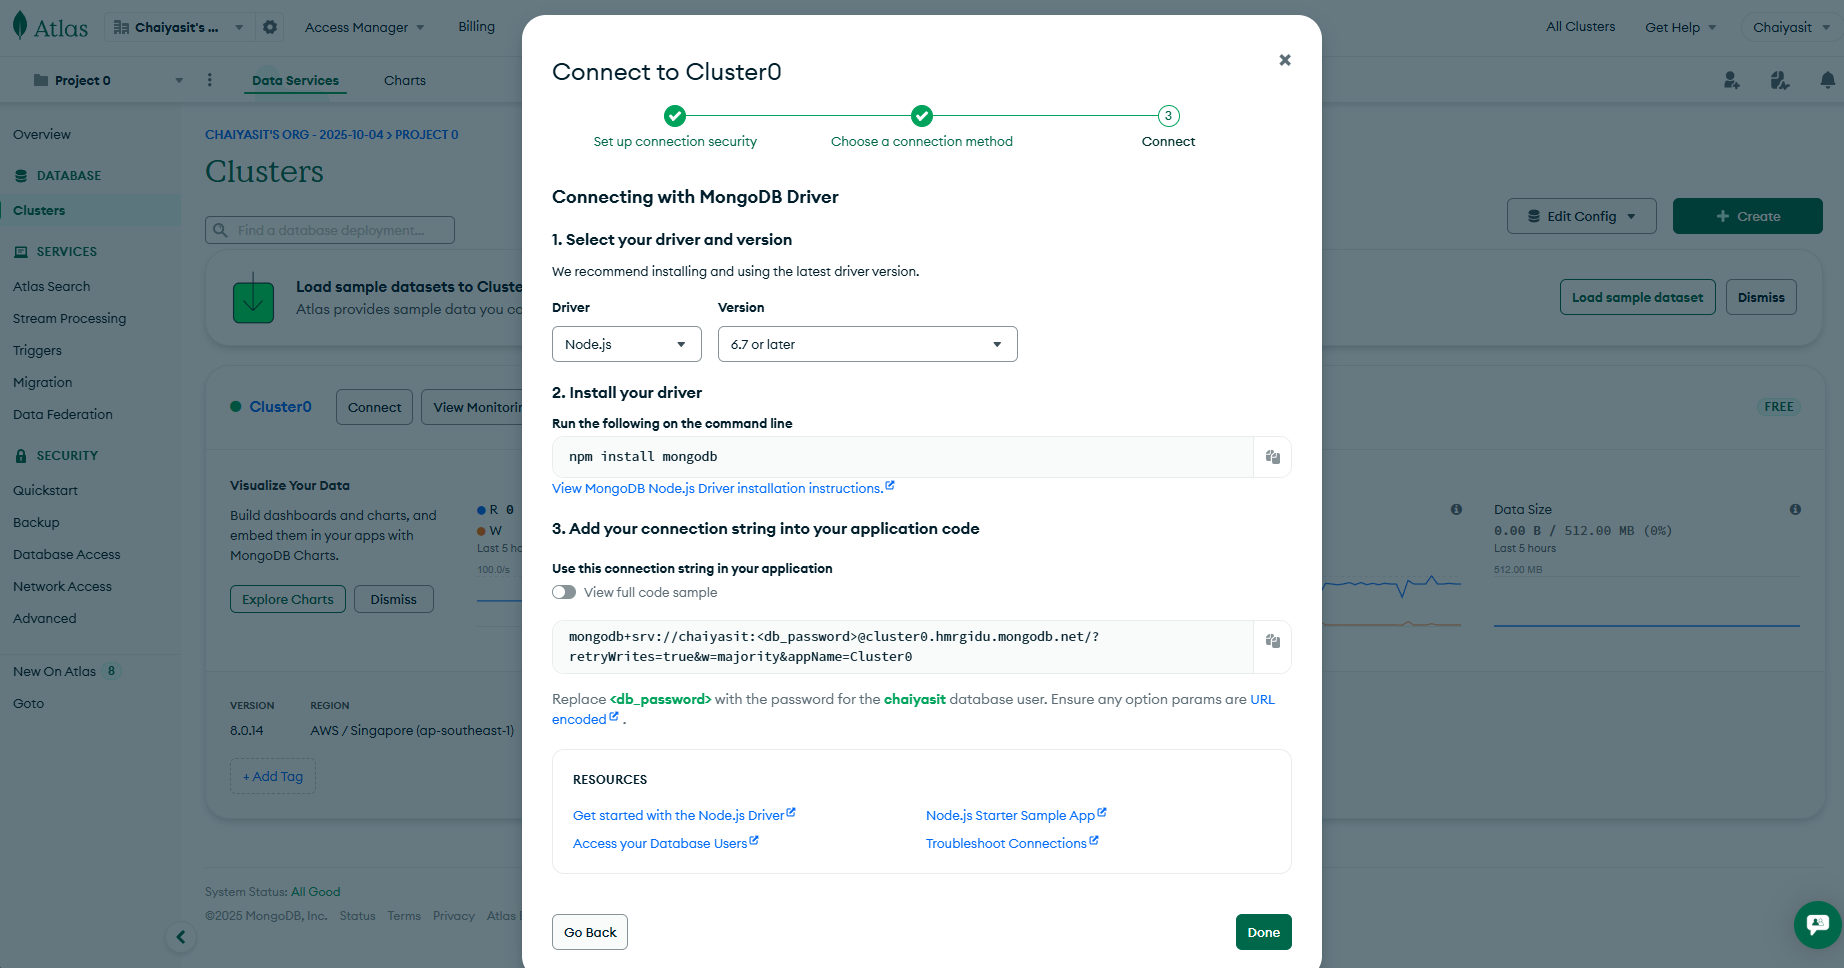
\includegraphics[width=1.0\textwidth]{Image/mongodb-use2.png}
}
\caption{\fontSixTeen{หน้าสำหรับเลือกวิธีการเชื่อมต่อกับ Cluster}}
\label{figA:WebSiteMongoDB16}
\end{figure}
    \item จากภาพที่ \ref{figA:WebSiteMongoDB16} ให้เลือก Drivers จากนั้นเลือก Node.js และเลือกเวอร์ชันที่ต้องการใช้ จากนั้นก็จะพบกับหน้าจอดังภาพที่ \ref{figA:WebSiteMongoDB17}   

\begin{figure}[H]
\centering
\adjustbox{frame, width=1.0\textwidth}{
    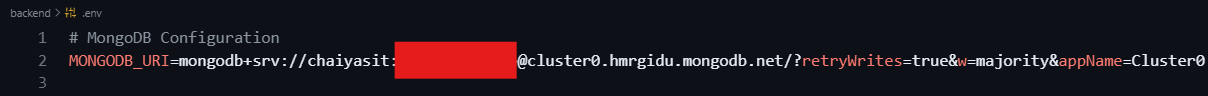
\includegraphics[width=1.0\textwidth]{Image/mongodb-use3.png}
}
\caption{\fontSixTeen{หน้าตัวอย่างการเชื่อมต่อกับ Cluster กับโปรแกรมผ่าน Connection String}}
\label{figA:WebSiteMongoDB17}
\end{figure}
    \item จากภาพที่ \ref{figA:WebSiteMongoDB17} คัดลอก Connection String ที่แสดงในภาพที่ จากภาพที่ \ref{figA:WebSiteMongoDB16}ไปใช้ในการเชื่อมต่อกับ Cluster ในโปรแกรม

\end{mycustomenum2}